\documentclass[aspectratio=169, 8pt]{beamer} % Reduced font size to 8pt

\usepackage[utf8]{inputenc}
\usepackage[T1]{fontenc}
\usepackage{helvet} % Standard proxy for consulting geometric sans
\usepackage{tcolorbox}
\usepackage{booktabs}
\usepackage{tikz}
\usepackage{pgfplots}
\pgfplotsset{compat=1.18}
\usepackage{graphicx}

% BCG-style Color Palette
\definecolor{bcgGreen}{RGB}{0, 114, 54}       % Classic BCG Green
\definecolor{bcgDarkGray}{RGB}{60, 60, 60}    % Deep Gray for body text
\definecolor{bcgLightGray}{RGB}{240, 240, 240} % Light gray for backgrounds
\definecolor{bcgTeal}{RGB}{0, 142, 116}       % Secondary teal

% Beamer Theme Settings (Minimalist / BCG style)
\setbeamertemplate{navigation symbols}{}
\setbeamercolor{frametitle}{fg=bcgDarkGray, bg=white}
\setbeamercolor{title}{fg=bcgDarkGray}
\setbeamercolor{normal text}{fg=bcgDarkGray}
\setbeamercolor{itemize item}{fg=bcgGreen}
\setbeamercolor{itemize subitem}{fg=bcgTeal}
\setbeamercolor{author}{fg=bcgDarkGray}
\setbeamercolor{date}{fg=bcgDarkGray}

% BCG Action Title Format (Left aligned, line underneath, safe bounding)
\setbeamertemplate{frametitle}{
    \vspace{0.4cm}
    \begin{beamercolorbox}[wd=0.96\paperwidth,leftskip=0.2cm]{frametitle}
        \usebeamerfont{frametitle}\textbf{\insertframetitle}\\[0.1cm]
        \textcolor{bcgGreen}{\rule{\linewidth}{1.5pt}}
    \end{beamercolorbox}
    \vspace{-0.4cm} % Aggressively pull content up after title
}
\setbeamerfont{frametitle}{series=\bfseries, size=\large}

% Footer
\setbeamertemplate{footline}{
  \leavevmode%
  \hbox{%
  \begin{beamercolorbox}[wd=.333333\paperwidth,ht=2.25ex,dp=1ex,left]{}%
    \hspace*{0.5cm} \footnotesize \color{gray} Majid Mumtaz | Strategic Advisory
  \end{beamercolorbox}%
  \begin{beamercolorbox}[wd=.333333\paperwidth,ht=2.25ex,dp=1ex,center]{}%
    \footnotesize \color{gray} Strictly Private \& Confidential
  \end{beamercolorbox}%
  \begin{beamercolorbox}[wd=.333333\paperwidth,ht=2.25ex,dp=1ex,right]{}%
    \color{bcgGreen}\textbf{\insertframenumber{}} \hspace*{0.5cm} 
  \end{beamercolorbox}}%
  \vskip4pt%
}

\begin{document}

% Slide 1: Title
\begin{frame}[plain]
    \vspace{1.5cm}
    {\huge \textbf{\color{bcgDarkGray} Strategic Audit \& Governance Advisory}} \\ \vspace{0.4cm}
    {\Large \color{bcgGreen} Board-Facing Assurance for Complex Operating Environments} \\ \vspace{0.8cm}
    
    {\normalsize \textbf{Majid Mumtaz}, CIA, ACA, FCCA} \\
    {\small \color{gray} Dubai, UAE | Deployable Globally} \\ \vspace{0.2cm}
    {\small \color{gray} \href{mailto:majidrajpar@gmail.com}{majidrajpar@gmail.com} | \href{https://majidrajpar.github.io/portfolio_my}{majidrajpar.github.io/portfolio\_my}}
    
    \vspace{1cm}
    
\begin{tikzpicture}
        \draw[bcgGreen, very thick] (0,0) -- (2,0);
    \end{tikzpicture}
\end{frame}

% Slide 2: Core Mandates 1 & 2 + Graph
\begin{frame}{Standard audit sampling leaves capital exposed; targeted diagnostics and ML-driven assurance recover hard ROI}
    \begin{columns}[T]
        \begin{column}{0.55\textwidth}
            \begin{tcolorbox}[colback=bcgLightGray, colframe=bcgLightGray, arc=0pt, left=2pt, top=1pt, bottom=1pt]
                \textbf{\small \color{bcgGreen} Fraud \& Forensic Diagnostics}
            \end{tcolorbox}
            \textit{\scriptsize \color{gray} When the Board suspects leakage but standard testing returns clean.}
            \begin{itemize}
                \setlength{\itemsep}{1pt}
                \setlength{\parskip}{0pt}
                \item \textbf{Methodology:} Full population data extraction coupled with ML anomaly detection.
                \item \textbf{\color{bcgGreen} Quantified ROI:} Recovered \textbf{AED 7.7M} in a single engagement from the 95\% of transactions standard sampling missed.
            \end{itemize}
            
            \vspace{0.1cm}
            \begin{tcolorbox}[colback=bcgLightGray, colframe=bcgLightGray, arc=0pt, left=2pt, top=1pt, bottom=1pt]
                \textbf{\small \color{bcgGreen} Audit \& Governance Transformation}
            \end{tcolorbox}
            \textit{\scriptsize \color{gray} When internal audit acts as a compliance checkbox.}
            \begin{itemize}
                \setlength{\itemsep}{1pt}
                \setlength{\parskip}{0pt}
                \item \textbf{Methodology:} Restructuring legacy methodologies to align directly with commercial realities.
                \item \textbf{\color{bcgGreen} Quantified ROI:} Reduced critical fraud incidents by \textbf{78\%} during a period of 340\% transaction volume surge at a GCC holding group.
            \end{itemize}
        \end{column}
        
        \begin{column}{0.40\textwidth}
            \vspace{0.2cm}
            \begin{center}
            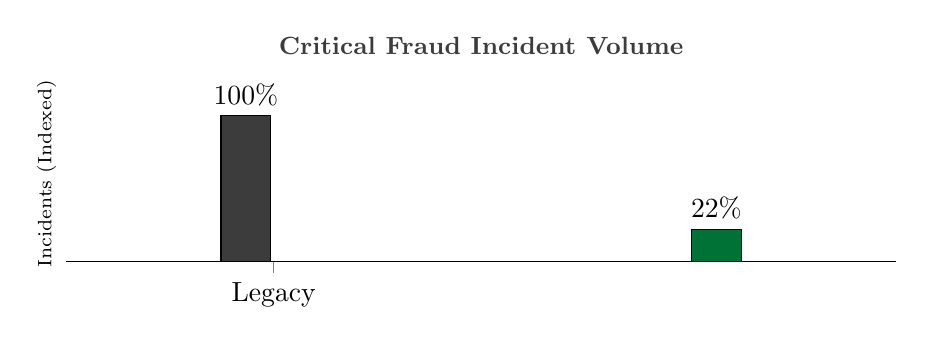
\begin{tikzpicture}
            \begin{axis}[
                ybar,
                width=\textwidth,
                height=3.8cm, % Aggressively compressed height
                bar width=18pt,
                enlarge x limits=0.5,
                ymin=0, ymax=120,
                ylabel={\scriptsize Incidents (Indexed)},
                symbolic x coords={Legacy, ML-Driven},
                xtick=data,
                nodes near coords={\pgfmathprintnumber\pgfplotspointmeta\%},
                nodes near coords align={vertical},
                axis lines*=left,
                y axis line style={opacity=0},
                ytick=\empty,
                title={\textbf{\small \color{bcgDarkGray} Critical Fraud Incident Volume}},
                title style={yshift=0.5ex}
                ]
            \addplot[fill=bcgDarkGray] coordinates {(Legacy,100)};
            \addplot[fill=bcgGreen] coordinates {(ML-Driven,22)};
            \end{axis}
            \end{tikzpicture}
            \end{center}
        \end{column}
    \end{columns}
\end{frame}

% Slide 3: Core Mandates 3 & 4 + Graph
\begin{frame}{Readiness mandates and ERM frameworks must be bulletproofed against underwriter scrutiny and cyber threats}
    \begin{columns}[T]
        \begin{column}{0.55\textwidth}
            \begin{tcolorbox}[colback=bcgLightGray, colframe=bcgLightGray, arc=0pt, left=2pt, top=1pt, bottom=1pt]
                \textbf{\small \color{bcgGreen} Pre-IPO \& M\&A Diligence}
            \end{tcolorbox}
            \textit{\scriptsize \color{gray} When preparing for capital markets or acquiring targets.}
            \begin{itemize}
                \setlength{\itemsep}{1pt}
                \setlength{\parskip}{0pt}
                \item \textbf{Methodology:} Rigorous stress-testing of ITGCs and governance frameworks against CMA standards.
                \item \textbf{\color{bcgGreen} Quantified ROI:} Uncovered \textbf{SAR 15M} in hidden exposures during buy-side due diligence, shifting negotiation leverage entirely.
            \end{itemize}
            
            \vspace{0.1cm}
            \begin{tcolorbox}[colback=bcgLightGray, colframe=bcgLightGray, arc=0pt, left=2pt, top=1pt, bottom=1pt]
                \textbf{\small \color{bcgGreen} Enterprise Risk \& IT Governance}
            \end{tcolorbox}
            \textit{\scriptsize \color{gray} When boards require quantifiable assurance over systemic exposures.}
            \begin{itemize}
                \setlength{\itemsep}{1pt}
                \setlength{\parskip}{0pt}
                \item \textbf{Methodology:} Board-commissioned ERM framework design and rigorous MSSP cybersecurity oversight.
                \item \textbf{\color{bcgGreen} Quantified ROI:} Designed an ERM framework that directly informed an insurance strategy overhaul, reducing premiums by \textbf{15\%}.
            \end{itemize}
        \end{column}
        
        \begin{column}{0.40\textwidth}
            \vspace{0.2cm}
            \begin{center}
            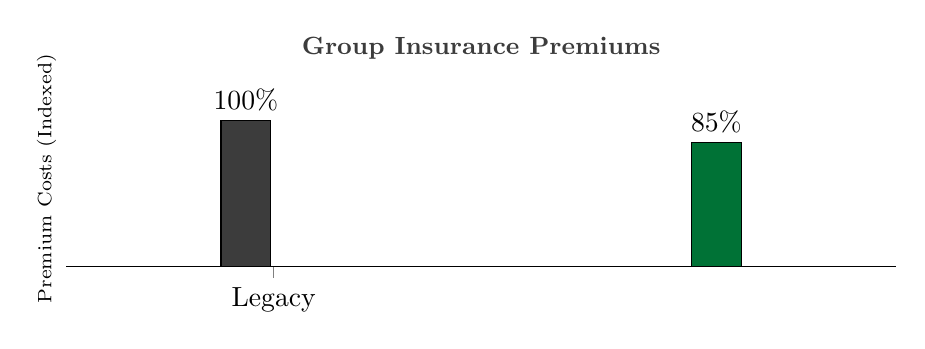
\begin{tikzpicture}
            \begin{axis}[
                ybar,
                width=\textwidth,
                height=3.8cm, % Aggressively compressed height
                bar width=18pt,
                enlarge x limits=0.5,
                ymin=0, ymax=120,
                ylabel={\scriptsize Premium Costs (Indexed)},
                symbolic x coords={Legacy, New ERM},
                xtick=data,
                nodes near coords={\pgfmathprintnumber\pgfplotspointmeta\%},
                nodes near coords align={vertical},
                axis lines*=left,
                y axis line style={opacity=0},
                ytick=\empty,
                title={\textbf{\small \color{bcgDarkGray} Group Insurance Premiums}},
                title style={yshift=0.5ex}
                ]
            \addplot[fill=bcgDarkGray] coordinates {(Legacy,100)};
            \addplot[fill=bcgGreen] coordinates {(New ERM,85)};
            \end{axis}
            \end{tikzpicture}
            \end{center}
        \end{column}
    \end{columns}
\end{frame}

% Slide 4: Thesis & Testimonials
\begin{frame}{Business Problem First, Controls Second: We design frameworks that reflect commercial reality, not just compliance}
    \vspace{-0.2cm}
    \begin{tcolorbox}[colback=bcgLightGray, colframe=bcgLightGray, arc=0pt, left=8pt, top=4pt, bottom=4pt]
    \textbf{\color{bcgDarkGray} The Operating Thesis:} A control that stops the business from operating is a failed control. I do not sell "best practice" compliance binders that gather dust. I build and audit controls that reflect commercial reality, utilizing automated data pipelines to monitor risk continuously without slowing down operations.
    \end{tcolorbox}
    
    \vspace{0.2cm}
    \textbf{\normalsize \color{bcgGreen} Endorsements from the Executive Suite}
    \vspace{0.1cm}
    
    \begin{columns}[T]
        \begin{column}{0.48\textwidth}
            \textit{\small ``Majid approaches complex matters with maturity and calm, and his recommendations are always grounded in a deep understanding of both risk and business impact. Any organisation—particularly within the F\&B or consumer space—would benefit greatly from his leadership.''} \\
            \vspace{0.1cm}
            \textbf{\footnotesize \color{bcgGreen} — Sally Swanepoel, Founder (Kitopi Colleague)}
        \end{column}
        \begin{column}{0.48\textwidth}
            \textit{\small ``His ability to bridge the gap between complex risk environments and practical, actionable business solutions is unmatched. Majid is a rare breed of auditor who actually understands how a business breathes.''} \\
            \vspace{0.1cm}
            \textbf{\footnotesize \color{bcgGreen} — Steve Skoien, CEO}
        \end{column}
    \end{columns}
\end{frame}

% Slide 5: Engagement Models
\begin{frame}{Flexible deployment models designed to solve immediate bottlenecks or provide sustained board-level assurance}
    \vspace{-0.2cm}
    Available for deployment via \textbf{Catalant}, \textbf{Veritux}, or \textbf{Direct Independent Contract}.
    
    \vspace{0.3cm}
    \begin{itemize}
        \setlength{\itemsep}{10pt}
        \item \textbf{\normalsize \color{bcgDarkGray} Targeted Diagnostics \color{bcgGreen}(2–4 Weeks)} \\
        Intensive sprints to validate a specific risk or forensic suspicion using full-population data extraction and ML modeling.
        
        \item \textbf{\normalsize \color{bcgDarkGray} Transformation Projects \color{bcgGreen}(3–6 Months)} \\
        Extended mandates to rebuild governance frameworks, set up whistleblowing channels, or prepare an organization for an IPO.
        
        \item \textbf{\normalsize \color{bcgDarkGray} Fractional CAE Advisory \color{bcgGreen}(Ongoing)} \\
        Retained, board-level assurance for family offices and holding groups needing senior oversight without a full-time overhead.
    \end{itemize}
\end{frame}

\end{document}
